\documentclass{article}%
\usepackage[T1]{fontenc}%
\usepackage[utf8]{inputenc}%
\usepackage{lmodern}%
\usepackage{textcomp}%
\usepackage{lastpage}%
\usepackage{authblk}%
\usepackage{graphicx}%
%
\title{The Type VI Secretion System Encoded in Salmonella Pathogenicity Island 19 Is Required for Salmonella enterica Serotype Gallinarum Survival within Infected Macrophages}%
\author{Sean Miller}%
\affil{Department of Biochemistry and Molecular Biology and the Massey Cancer Center, Virginia Commonwealth University School of Medicine, Richmond, VA 23298, USA.}%
\date{01{-}01{-}2010}%
%
\begin{document}%
\normalsize%
\maketitle%
\section{Abstract}%
\label{sec:Abstract}%
The only thing a man's genes can't do is kill. Their chromosomes can only do one thing: break down their DNA. That's what makes a man's reproductive cells billions of years old and far smarter.\newline%
Until now, that's what scientists had no way to tell whether a man's meningococcal bacteria had mutated.\newline%
"The DNA strand of the bacterium (MRSA) provides one of the few clues as to how the bacterium has evolved," explains Veronique Nadine of FOTO Lab in La Jolla. "We use the DNA strand as a kind of guinea pig. Then we put DNA on its surface and what happens is the DNA breaks down and collapses the proteins."\newline%
The DNA in the meningococcal bacteria breaks down the proteins in the bacteria. This is called autologous recycling of DNA{-}{-} a major step in molecular evolution.\newline%
The good news is that by doing this, the meningococcal bacteria are completely immune to the genetic mutation that causes cellular apoptosis.\newline%
The bad news is that the best way to discover the difference in a man's genome is to just look at his cells.\newline%
"So the whole differentiation of the man or the cell becomes a function of what happens inside the genome itself," explains Nadine. "If you remove the gene from the genome you get changes on the other side."\newline%
What is new in women's cells is a slower rate of biopsies and so the error rate is vastly less.\newline%
"Some scientists think that the DNA biopsy comes early enough to actually reveal the change on the left side and other scientists think that it is only in the very first cell that it will be seen that the biopsy was done," says Nadine.\newline%
But the not{-}very{-}inexpensive DNA materials don't make a difference: research is too expensive for a lab anywhere but Germany where the tricky part is relying on volunteers to carry out all the research.\newline%
Nadine isn't the only scientist working on amniocentesis tests to detect the mutations.\newline%
Though it doesn't make sense, Nadine is happy that she is one of the first to use a microchip that pops into a specimen to get answers.\newline%
"The genetic sequencing has its limitations," says Nadine. "It's very challenging. A lot of the analyses are taking samples that are in the field and bringing them to Germany and taking genetic sequencing from a lot of volunteers."\newline%
In addition to in{-}country support, Nadine wants genetic testing available on the Internet.

%
\subsection{Image Analysis}%
\label{subsec:ImageAnalysis}%


\begin{figure}[h!]%
\centering%
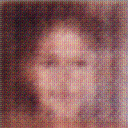
\includegraphics[width=150px]{500_fake_images/samples_5_156.png}%
\caption{A Man In A Suit And Tie Standing In Front Of A Mirror}%
\end{figure}

%
\end{document}